\section{Model View Controller}\label{sec:mvc}
The Model View Controller (MVC) is a design pattern widely used in programming to separate the program into different layers called `Model', `View', and `Controller'.
This provides the advantage that the structure gains clarity and becomes easier to maintain as it separates responsibility to individual layers, and is why this design pattern is used.

An illustration of MVC can be seen in \figref{fig:MVC}.
\begin{figure}[h]
	\centering
	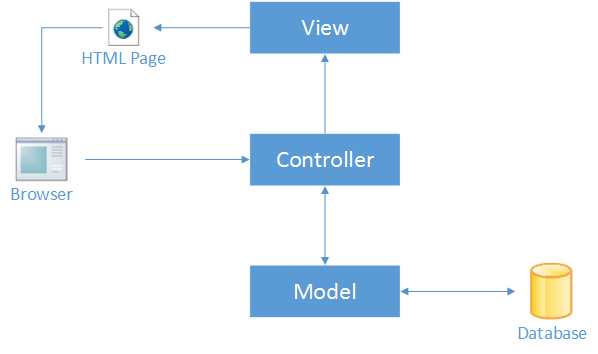
\includegraphics[scale=0.6]{relevantmaterial/MVC}
	\caption{Illustration of the MVC pattern.}\label{fig:MVC}
\end{figure}

The `Model' layer provides abstraction over the data stored in the database.
Additionally it provides business logic to work on this data and functions to modify the state of the database.

A request from the browser is interpreted into a controller action.
The `Controller' provides a set of 'actions' that can be executed based on the interpretation of the browser request. 
These actions then use functions in the `Model' layer and uses views to show an representation of the model, e.g. a table or a map of stations. 
These views are then presented to the user through the browser.
A controller may include multiple views to get a HTML page generated for the client to view.
As multiple views may be included by the controller, it may use separate views for the header, the body, and finally one for the footer. 
These multiple views allow for reuse of views and is also well suited for asynchronous loading of smaller parts of a page.

It is important to note that there is a single model layer, consisting of multiple entities (e.g bicycle and booking) and their associated services.
Additionally, it is a good practice to have multiple controllers, which each handle different parts of the website.
An example is to have a home and user controller.
With the user controller taking care of everything connected to user login, editing of profile, logout etc. and some actions could be moved to a separate controller if it becomes unmanageable.
The home controller takes care of the presentation of the frontpage.
To ensure better code clarity, the controllers are split into different responsibility areas of the website, each such controller containing a set of actions related to its responsibility area.

In addition to the better code clarity, as the website is organised in the way it is, working with the same model, the layout of the website can easily be changed, by including other views or developing additional controllers for other work routines.
This is related to the high modularity you gain with the MVC pattern, leading to high cohesion (elements in a module belong together to a high degree) and low coupling (low interdependence between modules).

However, some things need to be loaded asynchronously for increased usability, which is where AJAX comes in.